%preamble
% \documentclass{article}
\documentclass[journal]{IEEEtran}

%sets length of spacing between paragraphs
% \setlength{\parskip}{1em}

\usepackage[hidelinks]{hyperref}

\usepackage{graphicx}
\graphicspath{ {images/} }

\synctex=1

\usepackage{lipsum}
\usepackage{pgf-pie}
\usepackage{adjustbox}
\usepackage{float}
%title page
\title{Mass Effect 3 and Uniting the Galaxy in the Face of Total Destruction\\
\vspace{.25cm}\large ENGL 199 Research Report \vspace{-.5cm}}
\author{\LARGE Arun Woosaree}
\date{\today}
%actual document
\begin{document}
\maketitle %insert titlepage here
% Video games are often blamed for many social problems,
% from laziness and lack of motivation to accomplish anything, to pent up aggression that gets released as acts of violence in the real world. Although the gameplay in the Mass Effect Series contains violence, by allowing the player to develop his/her own character, the narrative of the game causes players to think about societal issues such as inter-alien racism, and to resolve these issues in a civil manner.
\begin{abstract}
 Video games are often blamed for many social problems,
 from laziness and lack of motivation to accomplish anything, to pent up aggression that gets released as acts of violence in the real world. Although the gameplay in the Mass Effect Series contains violence, by allowing the player to develop his/her own character, the narrative of the game causes players to think about social issues such as inter-alien racism, and to resolve these issues in a civil manner.
\end{abstract}

% \LaTeX{} IEEE style:
% %ieee style help:
% \url{https://www.overleaf.com/15366912ngxtshbtbmhm#/58219789/}
%Introduction
% \textbf{Conflicts to talk about:}
% \begin{itemize}
%  \item Krogans and Salarians - Genophage
%  \item working with the council against Cerberus. Cerberus is basically a pro human hate group analagous to white supremists today
%  \item Quarians and geth - is synthetic life important?
% \end{itemize}
% -reapers- exterminate all organic life in a cycle every 50,000 years
% \\ \\
% \textbf{Statistics:}
% \begin{enumerate}
%  \item 92\% of players cured the genophage
%  \item 64.5\% chose the paragon(good) options and 35.5\% the more mean shepard - can be the `no' part of the qualified argument for paragraph 1
%  \item 27\% choose to save the quarians, 37\% the geth, and 36\% both
% \end{enumerate}
% \\ \\
% \textbf{Outline:}
% \begin{itemize}
%  \item Introduction:
%        \begin{itemize}
%         \item general statement (importance of the topic)
%         \item thesis sentence (opinons and why, make a qualified argument)
%        \end{itemize}
%  \item Body paragraphs: Start with the concession , then continue with arguments supporting your opinion
%        \begin{enumerate}
%         \item No
%         \item Yes
%         \item Yes
%        \end{enumerate}
%
% \end{itemize}
% ...with over 88.3 million hours spent by players in the single player campaign.\cite{ea}...
%
%
% The narrative takes place in the future, where humans are no longer concerned about racism amonsgt themselves but rather societal
% tensions are between alien races. (If anything there are ideological tensions ie. with cerberus and the alliance but these
% tensions are not a result of racism amonsgt humans, but rather different ideological views of what is the best interest for the human race. (cerberus believes in using any methods (even illegal and terrorist like) for furthering the human race.)
% both organizations goals are to ultimately do what they believe is best for the entire human race). Rather, racial tensions are observed betweeen different alien races.
% \\ \\ \LARGE{\textbf{k, report actually begins below:}}
% \normalsize
\section{Introduction}
Although video games are commonly criticized for promoting aggression, and desensitising indivuduals, Mass Effect touches on some very important %societal
social issues today, by making the player think about political views,
and what stances they should pick. One of the prevalent issues in the world today is racism. In Mass Effect 3, the issue of racism is portrayed through alien characters, and tensions between them. The narrative takes place in the future, where humans are no longer concerned about racism amongst themselves. The ultimate goal of the game is to make (sometimes difficult) decisions as a representative for humanity, resolve diplomatic tensions, and unite the races against a common threat -the Reapers.

The Reapers are advanced synthetic life forms, which perform a purge of all intelligent organic life every 50,000 years in the Milky Way,
% which is
known as a `harvest'. They were made to preserve organic life, since
(within the Mass Effect universe), intelligent lifeforms, once advanced
enough to develop technological advancements ultimately make synthetic
lifeforms which rebel and destroy their organic creators. Ironically,
the solution to this problem in the Reapers' view is to harvest the genetic makeup of the galaxy, and allow new civilizations to grow and be harvested in a continuous cycle. The ultimate goal of the game is to unite the intelligent
races in the Milky Way Galaxy against the Reapers, and break the cycle.
However, the races must work together to do so,
and history tells that every previous cycle was
unsuccessful due to unresolved conflicts between the intelligent races, resulting in a lack of cooperation. The game puts the player in the position of Commander Shepard (male or female), who is tasked with making important decisions as a leader to unite the races using diplomacy, and to ultimately be the saviour of all organic life in the Milky Way Galaxy.

\section{Extremist Views - Cerberus Terrorist organization}
% \textit{Body paragraphs: Start with the concession , then continue with arguments supporting your opinion}
Although the primary goal in Mass Effect 3 is to unite the alien races, some
extremist views are presented, which the player can choose to side
with ideologically to some extent. Cerberus, led by the Illusive Man is
a xenophobic prohuman paramilitary group \cite{chrisb}\cite{wikia}
who believe that earth's government, the Systems Alliance is too
worried about law, and public opinion to stand up to other Citadel races.
The Citadel is a United Nations like coalition of the intelligent races in the Milky Way. Cerberus believes that ``any methods of advancing humanity's ascension are entirely justified, including illegal or dangerous experimentation, terrorist activities, sabotage and assassination.''\cite{wikia}
Cerberus's claim that it promotes the rights of humans, despite being
essentially a hate group for other aliens is strikingly similar to
extremists today, who also engage in illegal activities
to promote their agendas.
% Opportunities are presented to the player to agree with some of the
% Illusive Man's actions.
One of
Cerberus's main goals is to control Reaper technology to gain a technological
advantage for humans. However, the means for doing so are widely regarded as unacceptable. At one point in the narrative, it is found that Cerberus
had been running a ``Sanctuary'', wherin people seeking
shelter from the Reapers were taken in and used as human test subjects
subject to torture and premature death. Commander Shepard is given the opportunity to agree with the Illusive Man that the Reapers should be controlled, but if the player so chooses, the Illusive Man denies.
It can be noted that the wrecklessness of the experiments run by Cerberus
appear to be analagous the type of human experimentation run in
Nazi Germany, having to do with amputations, physical and mental trauma, and mutations.

Although the player is given the option to agree with the Illusive Man that Reapers should
be controlled instead of destroyed, Commander
Shepard does not join sides with Cerberus, since his goal is to save life.
Therefore, while the player is exposed to extremist views in the game,
it is made abundantly clear through storytelling and causing the player to feel
emotions such as disgust, and sympathy for the victims that the actions taken by Cerberus are morally wrong. The game shows that the end does not necessarily justify
the means, even if the player goes with the Renegade, or ruthless playing style
as a leader.


\section{Renegade and Paragon Playing Styles}
Throughout Mass Effect 3, the choices given to the player often fall into one
of two categories: Renegade and Paragon. The Renegade and Paragon system in
Mass Effect allows players to choose from one of two main playing styles.
The Paragon options typically have to do with showing compassion, or charming someone while Renegade choices are typically used for intimidation or coercion.
In this way, the game differentiates good choices of ``good'' and ``bad'',
with both options having positive and/or negative consequences.
Some would argue that the system, which allows players to choose Renegade options reinforces negative behaviours such as insulting people and/or intimidation. The game, in this regard allows the player to define their political views with regard to religion, views on other alien races,
and sexuality, with Renegade options tending to be less tolerant of some
alien races, religion, or extraterrestrial sexuality for example.
In contrast, players who choose Paragon options tend to solve issues by being more open and friendly to non playable characters, doing heroic actions, and
persuing justice for  victims. Fortunately, according to
statistics for Mass Effect 3 compiled in 2013 \cite{ea}, most players choose
to be a kind leader by making Paragon choices, which shows that the emotions
developed in the narrative generally make the player feel like they should
do the right thing.

\begin{figure}[h!]
 \centering
 
\includegraphics[width=.485\textwidth]{paragon}
 \caption{Most players choose on their own accord to be a kind leader as opposed to a ruthless one who gets the job done. \cite{ea}}
\end{figure}

As for the 35.5\% who chose the Renegade playing style, it should be noted that even if the player chooses to be a ruthless leader, the result of the player's actions are still for the greater good of the universe, which is saving
all life in the Milky Way from the threat of reapers. Furthermore, when choosing Renegade options, the player often sees the results of their actions,
which in some cases results in emotional responses from players who may even regret their actions, in spite of these events happening in a virtual world.
% \lipsum[3-4]

%Reason 2
\section{Tensions Between the Krogan and the Salarians}

Similar to today's world, there are races in Mass Effect who have a
long running grudge against each other for something done in the past.
The Krogans, a race of extremely tough reptilian bipeds used to
have a very high birth rates, and were colonising planets including those
of other nations in the Council. In retaliation, a biological weapon
called the Genophage, created by an amphibian race called the Salarians was unleashed on the Krogan.
This virus significantly reduced the
probablity of viable pregnancies of the Krogan race to 1 in 2000 \cite{wikia} ,
which left the Krogan vulerable to extinction. Understandably, the Krogans
were upset about the genocide and demanded a cure. However, the Salarians generally believed that the Krogan race was irresponsible, and that they did not deserve a cure. As a leader whose goal is to unite the races and gain military support to fight the Reapers,
difficult decisions must be made with what position to take. On a mission
to deploy a cure for the Genophage, the Salarian political leader contacts
Commander Shepard, offering military assets if the cure is sabotaged. On the
other hand, if the cure is administered, the Krogan offer their military support
in the struggle against the Reapers. As an outsider, it is easy to see that that while the Krogans did not have the right to conquer planets belonging to other races of the Council, the punishment (genocide) was too harsh and inhumane. In addition to facing extinction, younger Krogan are discriminated against by other races in
the Council, due to
the actions of their predecessors.
% their physical looks and stereotypes.
In player statistics revealed by Electronic Arts in 2013, 92\% of the players choose to cure the genophage \cite{ea}, which
\begin{figure}[h!]
 \centering
 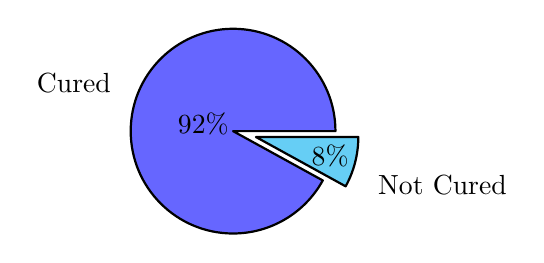
\begin{tikzpicture}
  \pie[pos={8,8},radius=1.3,explode =0.15]  {92/Cured, 8/Not Cured}
 \end{tikzpicture}
 \caption{Most players chose to cure the genophage \cite{ea}, an important diplomatic step for righting the wrongs of the Salarians.}
\end{figure}
may be a surprise to some, given that 35.5\% of players chose Renegade decisions. This implies that even those who
chose to play as a ruthless leader still found value in righting a wrong from
the past, even though the humans were not responsible for the mistake
made by the Salarians.
% In order to sabotage the cure,
% the player must make the choice of shooting Mordin (or try to convince him which usually is not successful because the ability to convince him depends on a lot of previous decisions made), an admirable character
% who previously worked on the Genophage and seeks to right his wrongs from the past
Even though the Salarians initially disapprove the cure for the Genophage,
the player can still gain the support of the Salarians later on. If the player chooses to sabotage the cure, however, the Krogans find out later, and military strength is reduced. Additionally, some would argue that it is heartbreaking to see a race facing extinction have hope for a cure to the disease killing them, only to have the cure sabotaged. In this way, the game reinforces the idea of ``doing the right thing'', and shows how strong racial tensions can be resolved using diplomacy.
% \lipsum[1-2]




%
% these alien races distrust each other because one developed a virus to wipe the
% other out.
% which is generally considered the ``good'' thing to do, since the Krogan have suffered due to this disease brought on them by the Salarians.
% ...this means that even a large portion of the 35.5\% who chose
% to be a ruthless leader still found value in the diplomatic implications
% of righting a wrong from the past, even if the mistake was not a cause
% of the human race. Furthermore, in an emotional moment where the Commander is
% presented with the choice to shoot Mordin, a young scientist who is dedicated
% to fixing the Genophage, only 4\% actually shot Mordin, even though shooting him would gain the military support of the Salarians. Even for the ruthless players, most of them could not justify shooting such an admirable character.
% %Reason 3
% \section{Are A.I. as important as Organic Life?}
% The Quarians, who developed machines called the geth to do work made these
% machines more advanced, and in violation of the Citadel's rules these machines
% become a fully blown self-aware Artificial intelligence. The Quarians attempt to wipe them out, but the geth retaliate, and the Quarians lose millions of people, and are now nomads, and lose representation on the Citadel.
% The player chooses between saving the Quarians, or gaining the military support of the geth, who have free will.

% Ultimately, at the end of the game, the player chooses between destorying
% all synthetic life, taking control of it, or merging organic and synthetic life,
% thus reaching the ``pinnacle of evolution''\cite{me}
% \lipsum[5-6]
% \adjustbox{margin=10}{}
% \begin{figure}
%  \begin{adjustbox}{width=.35\textwidth}
%   \begin{tikzpicture}
%    \pie[pos={8,8},radius=1,explode =0.05]  {27/Quarians, 37/Geth, 36/Both}
%   \end{tikzpicture}
%  \end{adjustbox}
%  \caption{Players appear to place as much value in synthetic life as in organic life. \cite{ea}}
% \end{figure}

%Conclusion
\section{Conclusion}
With over 88.3 hours played in single player campaign as of 2013 \cite{ea},
some would argue that Mass Effect 3 as a waste of time which
does not contribute to society in any meaningful way. However,
through the use of storytelling, the game reinforces positive social behaviours
and attitudes regarding social issues we experience today, such as racism.
By allowing players to make decisions, and develop emotional responses from the
consequences of their decisions,  Mass Effect 3 not only encourages ``good'' choices made by the player, but also allows the player to develop conflict resolution skills and resolving high-stakes issues through the use of diplomacy rather than violence, which may be one step towards fixing the issue of racism
in today's society.
%causes all references in the bib file to be cited, even though you don't mention them in the paper
\nocite{*}
\bibliographystyle{IEEEtran}
\bibliography{references}

\begin{figure}[]
 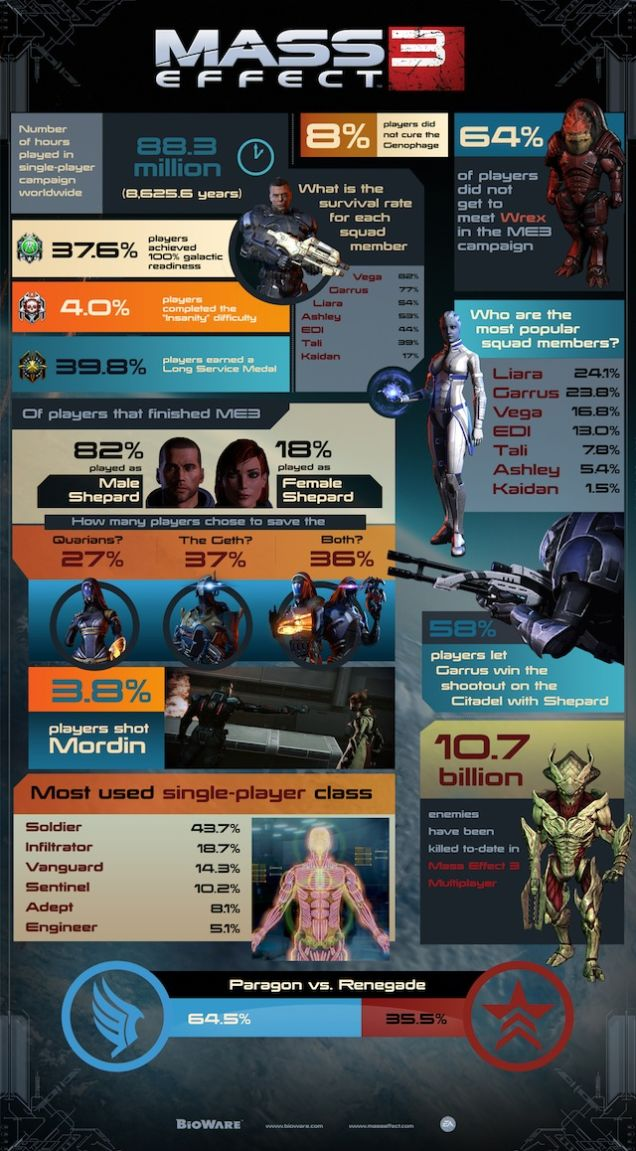
\includegraphics[width=.45\textwidth]{stat.jpg}
 \caption{Statistics referenced \cite{ea}}
\end{figure}
\end{document}
%URL={https://i.kinja-img.com/gawker-media/image/upload/18ie6sg7gatq8jpg.jpg}
